\documentclass[11pt]{article}
\usepackage[margin=1in]{geometry}
\usepackage{graphicx}
\usepackage{booktabs}
\usepackage{hyperref}
\usepackage{amsmath}
\usepackage{float}
\usepackage{subcaption}
\usepackage{enumitem}
\usepackage{multirow}

\title{DM2026 Assignment 2: Cross-Validation, SVM, Association Rules, and Clustering}
\author{Yu-Shun Liu \\ Student ID: 413551030}
\date{}

\begin{document}
\maketitle

\noindent\textbf{GitHub Repository:} \url{https://github.com/RaisoLiu/DM2026-Assignment-2}

%==============================================================================
\section{Q1: K-Fold Cross-Validation (15 pts)}
%==============================================================================

Continuation of Assignment 1 \texttt{Real\_World\_Classification.ipynb}, using the updated \texttt{linear\_model.py} from the course GitHub. The same preprocessing pipeline is reproduced: LabelEncoder on Species, KNNImputer($k=5$), train/test split (70/30, seed=40), and MinMaxScaler (fit on training data only).

\subsection{1(a) 5-Fold Cross-Validation: 4$\times$4 Hyperparameter Grid}

We perform 5-fold CV (\texttt{KFold(n\_splits=5, shuffle=True, random\_state=40)}) on the training set (350 samples) over 16 combinations of learning rate and L2 regularization strength. The model uses \texttt{n\_iteration=10000}, \texttt{val\_ratio=0.2}.

\begin{table}[H]
\centering
\caption{Mean CV accuracy for each (lr, $\lambda$) combination}
\begin{tabular}{lcccc}
\toprule
 & $\lambda=1.0$ & $\lambda=2.0$ & $\lambda=4.0$ & $\lambda=8.0$ \\
\midrule
lr=0.005 & 0.7200 & 0.7257 & \textbf{0.7314} & 0.7257 \\
lr=0.01  & 0.7257 & 0.7286 & 0.7286 & 0.7229 \\
lr=0.1   & 0.7171 & 0.7286 & 0.7257 & 0.7229 \\
lr=0.5   & 0.7171 & 0.6886 & 0.5229 & 0.4657 \\
\bottomrule
\end{tabular}
\end{table}

\subsection{1(b) Top 2 Hyperparameter Settings --- Test Evaluation}

The top 2 settings by CV accuracy are retrained on the full training set and evaluated on the held-out test set (150 samples).

\begin{table}[H]
\centering
\caption{Test evaluation for top 2 hyperparameter settings}
\begin{tabular}{llcccc}
\toprule
Rank & Setting & Accuracy & Precision & Recall & F1-score \\
\midrule
\#1 & lr=0.005, $\lambda$=4.0 & 0.7600 & 0.7273 & 0.8421 & 0.7805 \\
\#2 & lr=0.1, $\lambda$=2.0   & 0.7467 & 0.7215 & 0.7895 & 0.7540 \\
\bottomrule
\end{tabular}
\end{table}

\subsection{1(c) Observations}

\begin{itemize}
    \item \textbf{Small learning rates are robust to regularization strength.} Learning rates 0.005, 0.01, and 0.1 achieve similar CV accuracy ($\sim$72--73\%) across all $\lambda$ values, indicating that slow, stable convergence makes the model less sensitive to the regularization hyperparameter.
    \item \textbf{Large learning rate + strong regularization causes severe underfitting.} At lr=0.5, performance degrades sharply when $\lambda \geq 4.0$ (CV accuracy drops to 52.3\% and 46.6\%). When gradient steps are too large and regularization aggressively shrinks weights, the model cannot learn meaningful patterns.
    \item \textbf{Good generalization from CV to test.} The top-1 setting (lr=0.005, $\lambda$=4.0) achieves 73.1\% CV accuracy and 76.0\% test accuracy, and the top-2 setting generalizes similarly ($\sim$73\% $\to$ 74.7\%). This confirms that 5-fold CV on this dataset provides a reliable estimate of out-of-sample performance.
    \item The top-1 model shows higher recall (84.2\%) than precision (72.7\%), meaning it favors identifying positive samples at the cost of more false positives.
\end{itemize}

%==============================================================================
\section{Q2: SVM Classification (15 pts)}
%==============================================================================

We use the \texttt{mobile\_price.csv} dataset (2000 samples, 20 features, 4 balanced classes). Data is split 60/20/20 into train/validation/test sets (\texttt{random\_state=42}). F1-score uses \texttt{macro} averaging throughout.

\subsection{2(a) SVM with C=1.0}

\begin{table}[H]
\centering
\caption{SVM (C=1.0) performance across data splits}
\begin{tabular}{lcc}
\toprule
Set & Accuracy & F1 (macro) \\
\midrule
Train      & 0.9500 & 0.9505 \\
Validation & 0.9475 & 0.9463 \\
Test       & 0.9625 & 0.9617 \\
\bottomrule
\end{tabular}
\end{table}

\subsection{2(b) Performance vs.\ Regularization Parameter C}

We sweep $C \in \{0.001, 0.01, 0.1, 1, 10, 100, 1000, 10000\}$.

\begin{table}[H]
\centering
\caption{SVM performance for different C values}
\begin{tabular}{rcccccc}
\toprule
C & Train Acc & Train F1 & Val Acc & Val F1 & Test Acc & Test F1 \\
\midrule
0.001  & 0.2625 & 0.1040 & 0.2325 & 0.0943 & 0.2300 & 0.0935 \\
0.01   & 0.3242 & 0.2182 & 0.3075 & 0.2249 & 0.3000 & 0.2111 \\
0.1    & 0.8942 & 0.8959 & 0.8950 & 0.8949 & 0.9000 & 0.8987 \\
1      & 0.9500 & 0.9505 & 0.9475 & 0.9463 & 0.9625 & 0.9617 \\
10     & 0.9692 & 0.9696 & 0.9450 & 0.9442 & 0.9700 & 0.9693 \\
100    & 0.9775 & 0.9778 & \textbf{0.9550} & \textbf{0.9543} & 0.9700 & 0.9696 \\
1000   & 0.9867 & 0.9868 & 0.9500 & 0.9488 & 0.9700 & 0.9692 \\
10000  & 0.9975 & 0.9975 & 0.9400 & 0.9389 & 0.9700 & 0.9697 \\
\bottomrule
\end{tabular}
\end{table}

\begin{figure}[H]
\centering
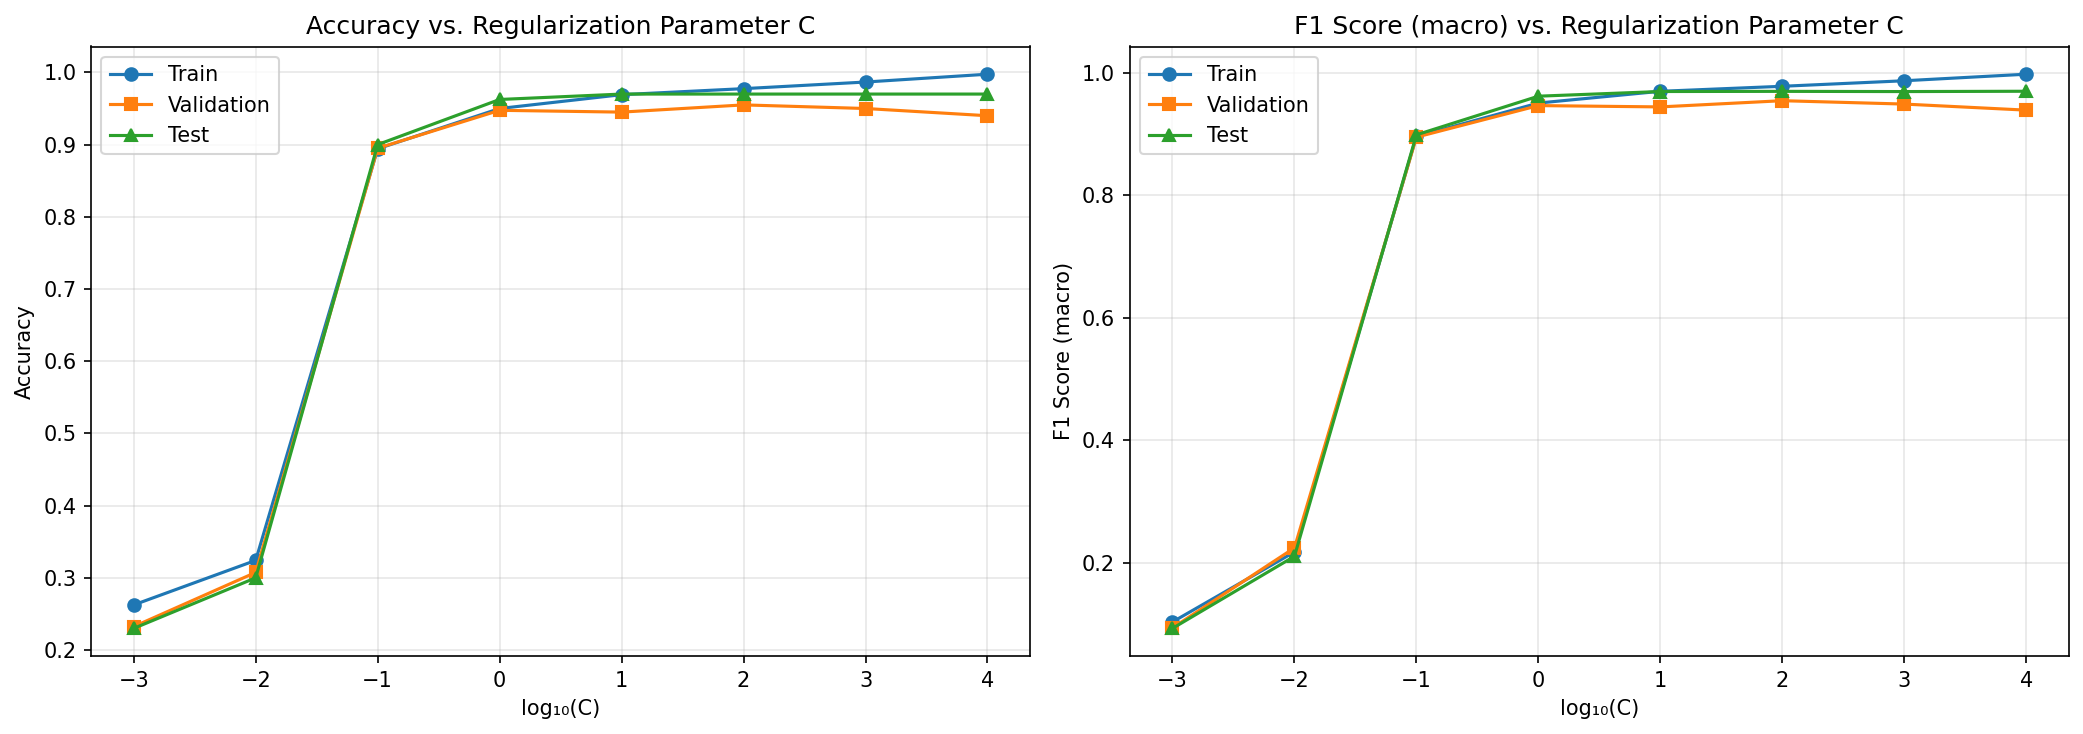
\includegraphics[width=\textwidth]{figures/q2_svm_c_sweep.png}
\caption{Accuracy and F1 score vs.\ $\log_{10}(C)$ for train, validation, and test sets.}
\end{figure}

\subsection{2(c) Best Generalization Performance}

\textbf{Best C = 100} (selected by highest validation accuracy = 95.5\%).

\begin{itemize}
    \item \textbf{Underfitting at small C:} With $C \leq 0.01$, the SVM's decision boundary is overly constrained, yielding accuracy near random chance (25\% for 4 classes). The margin is too wide and misclassifies most samples.
    \item \textbf{Optimal range:} Performance improves dramatically from $C=0.1$ ($\sim$89\%) to $C=1.0$ ($\sim$95\%). Beyond $C=1$, training accuracy continues climbing (reaching 99.8\% at $C=10000$) while validation accuracy peaks at $C=100$ (95.5\%) and then declines --- a classic overfitting signal.
    \item \textbf{C=100 balances fit and generalization:} The train--validation gap is moderate (2.25\%), and test performance is strong (97.0\% accuracy, 97.0\% F1). Although $C \in \{10, 1000, 10000\}$ achieve the same test accuracy, $C=100$ has the best validation score, making it the most reliable choice without peeking at test data.
\end{itemize}

%==============================================================================
\section{Q3: Association Rule Mining (15 pts)}
%==============================================================================

We filter samples with \texttt{price\_range == 1} (500 samples) and select 4 features: \texttt{ram}, \texttt{int\_memory}, \texttt{px\_width}, \texttt{battery\_power}. Each feature is discretized into low/medium/high using a 3:4:3 \textbf{value range} split:
\[
\text{low} \leq \min + 0.3 \times \text{range}, \quad
\text{medium} \leq \min + 0.7 \times \text{range}, \quad
\text{high} > \min + 0.7 \times \text{range}
\]

The discretized features are converted to a boolean one-hot transaction matrix ($500 \times 12$).

\subsection{3(a) Frequent Patterns (support $\geq$ 0.3)}

FP-Growth finds 8 frequent patterns:

\begin{table}[H]
\centering
\caption{Frequent itemsets with support $\geq$ 0.3}
\begin{tabular}{lc}
\toprule
Itemset & Support \\
\midrule
\{ram\_medium\} & 0.682 \\
\{px\_width\_medium\} & 0.416 \\
\{battery\_power\_medium\} & 0.414 \\
\{int\_memory\_medium\} & 0.412 \\
\{battery\_power\_medium, ram\_medium\} & 0.318 \\
\{int\_memory\_low\} & 0.316 \\
\{battery\_power\_low\} & 0.308 \\
\{ram\_medium, px\_width\_medium\} & 0.306 \\
\bottomrule
\end{tabular}
\end{table}

\subsection{3(b) Association Rules (support $\geq$ 0.3, confidence $\geq$ 0.4, lift $\geq$ 0.8)}

\begin{table}[H]
\centering
\caption{Association rules meeting all criteria}
\begin{tabular}{llccc}
\toprule
Antecedent & Consequent & Support & Confidence & Lift \\
\midrule
ram\_medium & battery\_power\_medium & 0.318 & 0.466 & 1.126 \\
battery\_power\_medium & ram\_medium & 0.318 & 0.768 & 1.126 \\
ram\_medium & px\_width\_medium & 0.306 & 0.449 & 1.079 \\
px\_width\_medium & ram\_medium & 0.306 & 0.736 & 1.079 \\
\bottomrule
\end{tabular}
\end{table}

\subsection{3(c) Observations}

\begin{itemize}
    \item \textbf{ram\_medium dominates:} 68.2\% of price\_range=1 phones have mid-range RAM, making it the most frequent single item and the anchor of both 2-item frequent patterns. This aligns with the second-lowest price tier having predominantly mid-range specifications.
    \item \textbf{Asymmetric confidence:} \texttt{battery\_power\_medium $\to$ ram\_medium} has 76.8\% confidence, while the reverse has only 46.6\%. This asymmetry arises because ram\_medium has much higher base support (68.2\%), so knowing a phone has medium battery power strongly predicts medium RAM, but not vice versa.
    \item \textbf{Mild positive associations:} All lift values are close to 1.0 (1.08--1.13), indicating that while medium-range features tend to co-occur slightly more than expected by chance, the associations are not dramatically strong. Within this price tier, the four features are somewhat independent.
    \item Only 2 two-item patterns and 4 rules pass all thresholds, reflecting the relatively uniform distribution of mid-range specifications in this price category.
\end{itemize}

%==============================================================================
\section{Q4: PCA and K-Means Clustering (20 pts)}
%==============================================================================

All 20 features from \texttt{mobile\_price.csv} are standardized using z-score (\texttt{StandardScaler}). The target variable \texttt{price\_range} (4 classes) is used only for evaluation, not for clustering.

\subsection{4(a) Standardization}

After \texttt{StandardScaler}, all features have mean $\approx 0$ and std $= 1$.

\subsection{4(b) PCA 2D Projection with True Labels}

\begin{figure}[H]
\centering

\includegraphics[width=0.75\textwidth]{figures/q4b_pca_true_labels.png}
\caption{PCA 2D projection colored by true price-range labels. The first two PCs explain only 16.5\% of total variance. Classes overlap heavily in this projection.}
\end{figure}

\subsection{4(c) K-Means on All Standardized Features}

\begin{figure}[H]
\centering
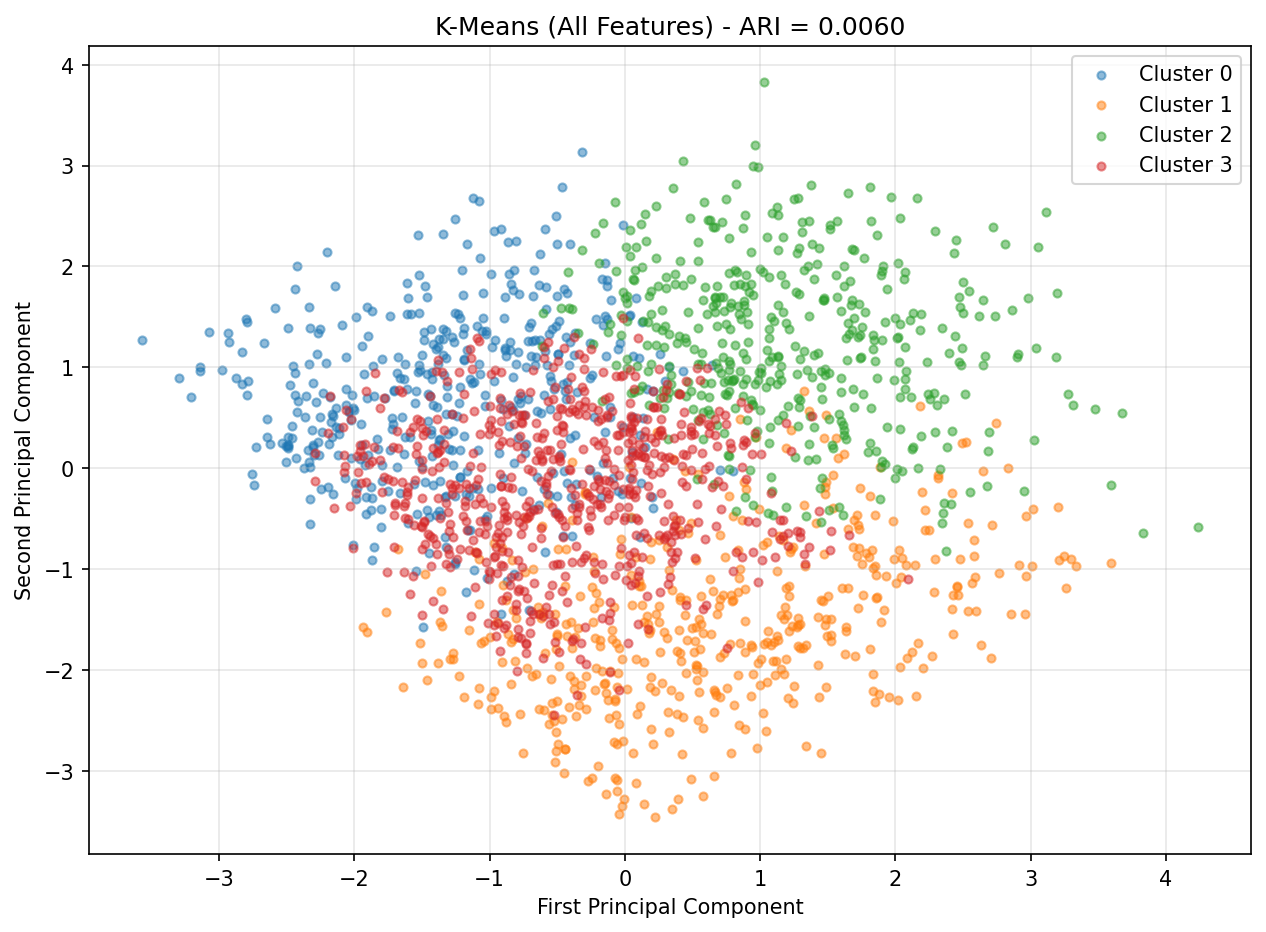
\includegraphics[width=0.75\textwidth]{figures/q4c_kmeans_all_features.png}
\caption{K-Means (all 20 features) visualized on PCA 2D plane. ARI = 0.0060.}
\end{figure}

\subsection{4(d) K-Means on PCA 2D Features}

\begin{figure}[H]
\centering
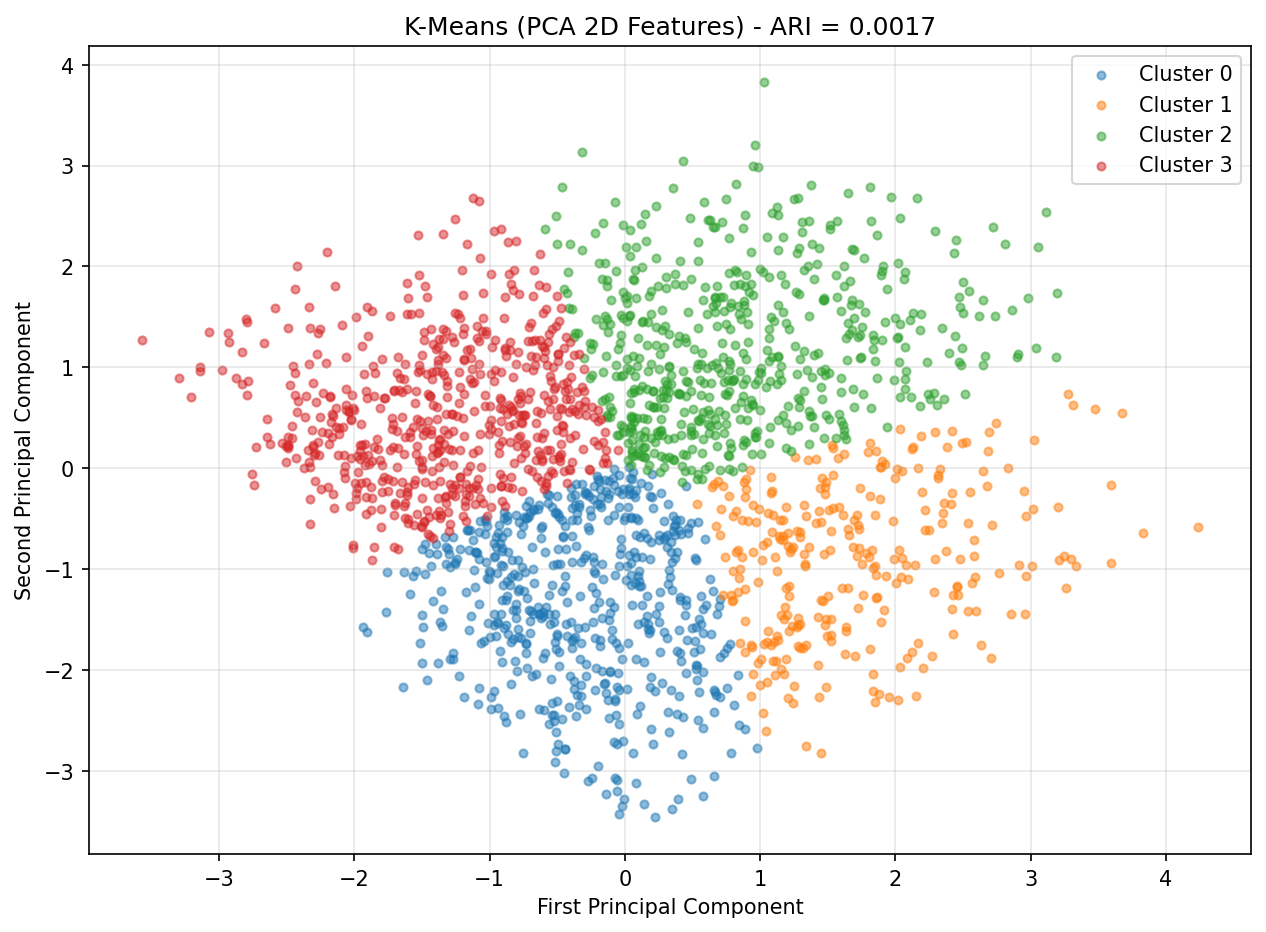
\includegraphics[width=0.75\textwidth]{figures/q4d_kmeans_pca_2d.png}
\caption{K-Means on PCA 2D features. ARI = 0.0017.}
\end{figure}

\subsection{4(e) Observations}

\begin{itemize}
    \item \textbf{PCA captures very little variance:} The first two principal components explain only 16.5\% of total variance. The 2D scatter plot shows heavy overlap among all 4 classes, indicating that the class structure is distributed across many dimensions rather than being concentrated in the top PCs.
    \item \textbf{Both K-Means approaches fail:} ARI values of 0.0060 (all features) and 0.0017 (PCA 2D) are near zero, meaning the clustering is essentially random with respect to the true labels.
    \item \textbf{Dimensionality reduction hurts slightly:} K-Means on all 20 features (ARI=0.0060) marginally outperforms K-Means on 2D PCA (ARI=0.0017), as expected since reducing to 2D discards 83.5\% of the variance.
    \item \textbf{K-Means is fundamentally unsuited here:} K-Means assumes spherical, equally-sized clusters in Euclidean space. The mobile price classes likely have complex, non-linear decision boundaries. This contrasts sharply with Q2's SVM results ($>$95\% accuracy), confirming that supervised methods with non-linear kernels (RBF) are necessary for this task.
\end{itemize}

%==============================================================================
\section{Q5: Enhancing K-Means with Association Rule Mining (35 pts)}
%==============================================================================

\subsection{Motivation and Approach}

Standard K-Means treats all features equally and ignores class-discriminative structure. We propose a two-pronged enhancement using association rule mining:

\begin{enumerate}
    \item \textbf{Rule-Guided Feature Weighting:} All features are discretized (3:4:3 value range split) and association rules are mined per class using FP-Growth (\texttt{min\_support=0.3}, confidence $\geq 0.5$, lift $\geq 1.0$). Features that appear frequently in high-lift rules across classes receive higher weights. The resulting weights range from 1.0 to 3.0 and are applied to the standardized features before clustering.
    \item \textbf{Class-Stratified Pattern Features:} The top 5 most discriminative patterns (ranked by lift $\times$ confidence) are selected from each class's rules, yielding 20 binary features. Each feature indicates whether a sample matches a specific class-associated itemset.
\end{enumerate}

The augmented feature matrix combines 20 weighted original features with 20 scaled pattern features (40 total).

\subsection{Evaluation Protocol}

Both baseline and improved K-Means are evaluated using the same protocol:
\begin{itemize}
    \item 5 random seeds: \{0, 10, 42, 100, 999\}
    \item \textbf{Hungarian algorithm} (\texttt{scipy.optimize.linear\_sum\_assignment}) maps cluster IDs to true labels optimally before computing accuracy, precision, recall, and F1 (all macro-averaged).
\end{itemize}

\subsection{Results}

\begin{table}[H]
\centering
\caption{Per-seed and average comparison of baseline vs.\ improved K-Means}
\begin{tabular}{clcccc}
\toprule
Seed & Method & Accuracy & Precision & Recall & F1 \\
\midrule
\multirow{2}{*}{0}   & Baseline & 0.2945 & 0.2940 & 0.2945 & 0.2926 \\
                      & Improved & 0.3885 & 0.4310 & 0.3885 & 0.3962 \\
\midrule
\multirow{2}{*}{10}  & Baseline & 0.2955 & 0.2953 & 0.2955 & 0.2936 \\
                      & Improved & 0.3905 & 0.4259 & 0.3905 & 0.3957 \\
\midrule
\multirow{2}{*}{42}  & Baseline & 0.2970 & 0.2966 & 0.2970 & 0.2950 \\
                      & Improved & 0.3885 & 0.4310 & 0.3885 & 0.3962 \\
\midrule
\multirow{2}{*}{100} & Baseline & 0.2955 & 0.2950 & 0.2955 & 0.2935 \\
                      & Improved & 0.3885 & 0.4310 & 0.3885 & 0.3962 \\
\midrule
\multirow{2}{*}{999} & Baseline & 0.2985 & 0.2984 & 0.2985 & 0.2956 \\
                      & Improved & 0.3885 & 0.4310 & 0.3885 & 0.3962 \\
\midrule
\multicolumn{2}{c}{\textbf{Average Baseline}} & 0.2962 & 0.2959 & 0.2962 & 0.2941 \\
\multicolumn{2}{c}{\textbf{Average Improved}} & \textbf{0.3889} & \textbf{0.4300} & \textbf{0.3889} & \textbf{0.3961} \\
\bottomrule
\end{tabular}
\end{table}

\begin{figure}[H]
\centering
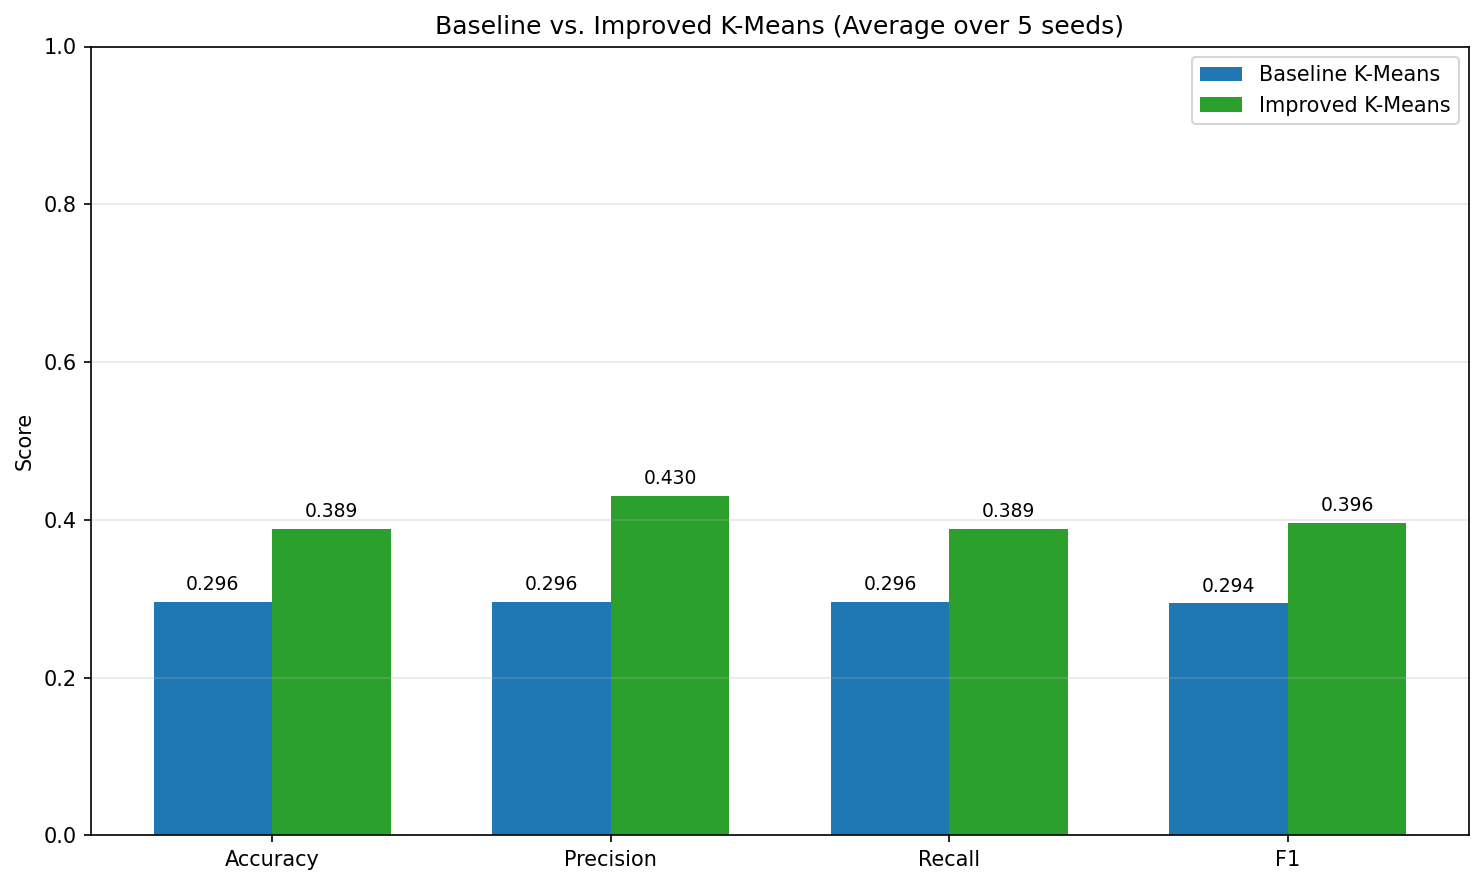
\includegraphics[width=0.75\textwidth]{figures/q5_comparison.png}
\caption{Average performance comparison across 5 seeds.}
\end{figure}

\subsection{Analysis}

\begin{itemize}
    \item \textbf{Consistent improvement:} The improved method outperforms the baseline across all seeds and all metrics. Average accuracy increases from 29.6\% to 38.9\% (+9.3 pp), and F1 from 29.4\% to 39.6\% (+10.2 pp). Precision sees the largest relative gain (29.6\% $\to$ 43.0\%).
    \item \textbf{Feature weighting is key:} Association rule mining reveals that \texttt{ram} (weight=3.0), \texttt{three\_g} (2.76), and \texttt{fc} (2.31) are the most class-discriminative features. Upweighting these features helps K-Means focus on dimensions that actually separate the price classes, rather than treating noise features equally.
    \item \textbf{Pattern features add structural information:} The 20 binary pattern features encode class-specific co-occurrence patterns (e.g., \{fc\_low, ram\_low, pc\_low\} for class 0; \{ram\_high, three\_g\_high, four\_g\_high\} for class 3). These features inject discrete structural knowledge that continuous features alone cannot capture.
    \item \textbf{Limitations:} Even with enhancement, 38.9\% accuracy remains far below the SVM's 97\%. K-Means is inherently limited by its assumption of spherical clusters and its unsupervised nature. The improvement demonstrates that association rule mining can meaningfully guide clustering, but cannot replace the power of supervised learning with non-linear kernels for this dataset.
    \item \textbf{Stability:} The improved method shows very low variance across seeds (std=0.0009 for accuracy), compared to baseline (std=0.0016). The rule-guided features create more consistent cluster structure.
\end{itemize}

\end{document}
